

\chapter{Using Deep Learning to Detect Technical Debt}

We aim to create a system that automatically detects technical debt in a class method. To achieve this goal, we took the following three steps: dataset creation, classification and hyperparameter tuning.
The dataset was automatically created by mining and processing open-source project histories. It's a balanced dataset by construction and the two classes are referred as: SATD and fixed.

We initially identify technical debt through the presence of SATD in the comments of the source code, using keyword labels pattern matching \cite{potdar2014exploratory} \cite{rantala2020prevalence}.
The identification of a SATD/fixed method pair is based on a strong assumption: when the SATD comment disappears, due to a commit, we suppose that the technical debt is fixed; so, we regard the new code as TD-free, i.e. belonging to fixed class.
% detail: describe the circumstances where we reject this hypotheses
The classifier is a neural network capable of representing snippets of code with an fixed length vector, conceptually similar on how word2vec works. The learned vector representation (code embedding) is associated with a semantic label (i.e. SATD or fixed).
Lastly, to increase the performance of the system we select a set of hyperparameters and perform a distributed grid search for tuning their values. The rest of this chapter explains each part in greater detail.

%3.1
\section{Mining SATD Instances and their Fixes}

These are the fundamental activities involved in the creation of the dataset:
\begin{itemize}
    \item Github repository url mining: using Github api, we extracted 248,872 projects' url matching our search profile.
    \item Repository cloning and filtering: some projects can be discarded only after the commit history is available for a precursory analysis to determine if a project qualifies for the next activity.
    \item Commit history processing: the directed acyclic graph of the commits is traversed and the source code is parsed in search of acceptable SATD/fixed pair.
\end{itemize}

The following sections describe these activities in detail.

\subsection{Github repository url mining}
% javaparser & pre-selection of repositories by api.


% Building a list of github repositories - github api tool -reject android repositories
% %mention the initial idea of specialization
% %remember --##string##--

% The process of cloning and caching repos.
% The source code processing. SATD search, exclusions, metrics (lines, tokens)
% Caching of code vectors.
% Parsing, comment cleaning, excluded patterns.
% SATD/fixed tracking. 
% Saving to h2 and then postgresql.

\subsection{Repository cloning and filtering}
\subsection{Commit history processing}
% the commit is like a function that transform the SATD in fixed
%3.2 
\section{The Deep Learning Model}
The model described in this section is called code2vec \cite{alon2019code2vec}.
The following three sequential processes can be considered a chain that progressively transform the source code into the desired target (i.e. the two classes SATD/fixed):
\begin{itemize}
    \item Decompose
    \item Aggregate
    \item Predict
\end{itemize}

\noindent Each of these steps can be viewed as a process that takes an input, creates an intermediate representation and generates an output for the next process.
In the rest of this section we give some details about each one of them and introduce some technical terms. 
\\
\\
\noindent \textbf{Decompose.} The input of this process is the source code. The output generated is a bag of path-context. The following list gives more detail on the process and the intermediate representations:

\begin{itemize}
    \item Parsing and creation of the abstract syntax tree of the method source code. 
    \item Extraction of all AST-paths (up to a fixed limit).
    \item Encoding of the AST-paths into a bag of context-vector.
    \item Transform each context vector into a path-context (so to obtain a bag of path-context).
\end{itemize}

\noindent \textbf{Aggregate.} This process aggregates the bag of path-context (the output from the previous process) using an attention vector. The final result is a code-vector that represents the snippet of code as continuous distributed vector, i.e. a `code embedding'.
\\
\\
\noindent \textbf{Predict.} The code-vector is feeded to a fully connected neural network that performs the classification using the desired classes (i.e. SATD/fixed).
\\
\\
\noindent In the following sections we expand and dig deeper in these concepts.

% Here I want to explain briefly what are the fundamental pieces and how they interact (without pretending that the reader really understands, but to give the general idea)

\subsection{Representing code using AST paths}
This section describes how to capture semantic information from a snippet of code and create a representation that can be used to predict properties of the snippet, for example a label (e.g. SATD/fixed).
To better illustrate how the decomposition is done we use as an example the simple code snippet in listing \ref{lst:snippet_ast_code}.

%AST of code snippet
\begin{lstlisting}[caption={Example code to show decomposition}, label={lst:snippet_ast_code},language=Java]

                            String METHOD_NAME() {
                              if(somePreCondition())
                                while(!completed())
                                   doWork();
                              return "ok";
                            }
                            
\end{lstlisting}

\noindent The abstract syntax tree (AST) is extracted from the source code using JavaParser \footnote{https://javaparser.org/}; see an example in figure  \ref{fig:AST_graphviz}.


% \begin{figure}
%  \centering
%  \resizebox{\columnwidth}{!}{
%  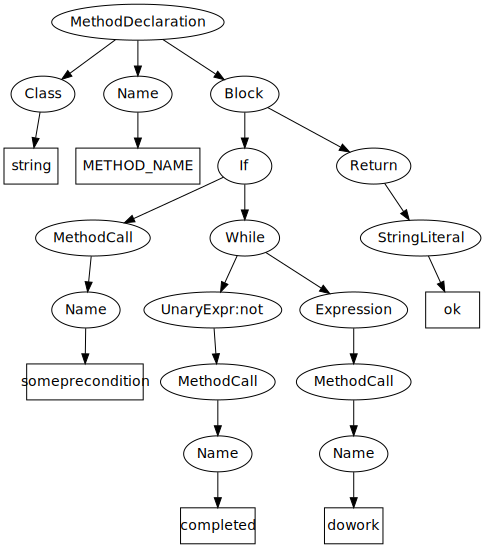
\includegraphics{images/AST-graphviz.png}
%  }
%  \caption[Encoder-Decoder model in a dialogue system application.]{Encoder-Decoder model in a dialogue system application. }
%     \label{fig:AST-graphviz}
% \end{figure}

\begin{figure}
 \centering
 \resizebox{\columnwidth}{!}{
%   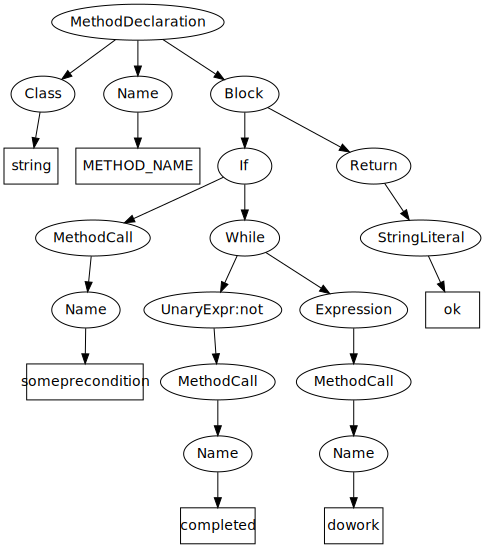
\includegraphics{images/AST-graphviz.png}
 %\includesvg[inkscapelatex=false]{images/AST-graphviz2}
 \includesvg[]{images/AST_graphviz}
%  \escapeus{\includesvg{images/AST_graphviz2.svg}}
%  \includesvg{images/AST-graphviz2.svg}
 }
 %[inkscapelatex=false,
 \caption[AST for listing \ref{lst:snippet_ast_code}.]{AST of listing \ref{lst:snippet_ast_code}.}
    \label{fig:AST_graphviz}
\end{figure}

	
We identify two sets of node in the AST: terminal and non-terminal nodes. Terminal nodes are the leafs and the rest are the non-terminal ones.
\textit{AST path definition}: it is a path connecting two terminal nodes and it must include one non-terminal node which is a common ancestor of the two terminal nodes. 
The representation of the program is the \textit{set of all its AST paths}. 

%AST paths of code snippet
\begin{figure}
 \centering
 \resizebox{\columnwidth}{!}{
  \includegraphics{images/AST_paths.png}
 }
 %[inkscapelatex=false,
 \caption[All AST paths for listing \ref{lst:snippet_ast_code}.]{AST paths of listing \ref{lst:snippet_ast_code}.}
    \label{fig:AST_paths}
\end{figure}

% \begin{lstlisting}[caption={All AST paths for listing \ref{lst:snippet_ast_code}}, label={lst:AST_paths}, basicstyle=\small,breaklines=true,inputencoding=utf8, extendchars=\true]

% \uparrow and \downarrow
% ↑

% \end{lstlisting}

% here I go into details on the first decomposition/representation of the code snippets into fixed length vectors

\subsection{Bag of path-contexts}

\subsection{Context-vector $c_i$}
%how many OOV? 
%https://github.com/tech-srl/code2vec/blob/c98e8f786b7262e56c93e520d039fb7aa5d0f7ef/vocabularies.py#L123

\subsection{Combined context-vector $\widetilde{c}_i$}

\subsection{Attention mechanism and the code-vector}

\subsection{Training and prediction}
% detailed explanations in step:
% - representation idea (ast, path learning)

% - semantic labeling

% - SATD/fixed

% The model used is called code2vec. The idea is to represents source code snippets using a fixed length vector i.e. code embedding. 
% The abstract syntax tree (AST) is used, there is an attention mechanism and it was successful in predicting semantic labeling.

% Simple and fast


%3.3
\section{Hyperparameter Tuning}

This section describes the process of tuning the hyperparameters of the model.

It is clear that using shorter code snippets increases the performance but decreases the number of samples in the dataset; thus decreasing the usefulness of the trained model because of less capability in generalization.
For the tuning of the hyperparameters, we empirically defined to keep those snippets with less than 200 tokens; an example of a method composed by 199 tokens is shown in listing \ref{lst:snippet199}.

\begin{lstlisting}[caption={Code snippet with 199 tokens}, label={lst:snippet199},language=Java]
private CompoundWorkflow finishCompoundWorkflow(
  WorkflowEventQueue queue,
  CompoundWorkflow compoundWorkflow, 
  String taskOutcomeLabelId, 
  String userTaskComment, 
  boolean finishOnRegisterDocument, 
  List<NodeRef> excludedNodeRefs) {
    if ((finishOnRegisterDocument &&
      compoundWorkflow.isStatus(Status.FINISHED)) ||
      (!finishOnRegisterDocument &&
      checkCompoundWorkflow(compoundWorkflow,
      Status.IN_PROGRESS, 
      Status.FINISHED) == Status.FINISHED)) {
        if (log.isDebugEnabled()) {
            log.debug("--##string##--" + compoundWorkflow);
        }
    } else {
        setWorkflowsAndTasksFinished(queue, compoundWorkflow, 
            taskOutcomeLabelId, userTaskComment,
            finishOnRegisterDocument, excludedNodeRefs);
        if (finishOnRegisterDocument || excludedNodeRefs != null) {
            stepAndCheck(queue, compoundWorkflow);
        } else {
            stepAndCheck(queue, compoundWorkflow, Status.FINISHED);
        }
        boolean changed = saveCompoundWorkflow(queue,
            compoundWorkflow, null);
        if (log.isDebugEnabled()) {
            log.debug("--##string##--" + compoundWorkflow);
        }
    }
    CompoundWorkflow freshCompoundWorkflow =
        getCompoundWorkflow(compoundWorkflow.getNodeRef());
        
    if (!finishOnRegisterDocument && excludedNodeRefs == null) {
        checkCompoundWorkflow(freshCompoundWorkflow, Status.FINISHED);
    }
    checkActiveResponsibleAssignmentTasks(
        freshCompoundWorkflow.getParent());
    return freshCompoundWorkflow;
}
\end{lstlisting}

\noindent \emph{-- Expand the following paragraph with more detail and graphs) --}

We inspected all the hyperparameters and set up a grid search using a tools called Optuna.
The hyperparameters subject of the distributed experiment are: embedding size, dropout keep rate and context length.
We run it with multiple GPU colab PROfessional and standards sessions. Both cpu and GPU. 

